\myChapter{Implementacja}\label{ch:implementation}
%************************************************

Jako zwolennik wolnego i otwartego oprogramowania starałem się korzystać tylko i wyłącznie z takich właśnie narzędzi.

\section{Oprogramowanie mikrokontrolera}
W pracy wykorzystany został układ \textsmaller{AVR Atmega8}, będący ośmiobitowym mikrokontrolerem. Sprzęt ten znacznie różni się od architektury znanej z komputerów osobistych \spacedallcaps{PC} i choć sama idea programowania jest podobna, wszystko pozostawione jest programiście, co w połączeniu z koniecznością programowania na bardzo niskim poziomie, jaki nie jest promowany na studiach, stanowi dodatkowe wyzwanie.

Oprogramowanie zostało stworzone w języku \texttt{C}, wykorzystując do kompilacji kompilator \textsmaller{avr-gcc} oraz bibliotekę \textsmaller{avr-libc}. Do programowania wykorzystałem program \textsmaller{avrdude}

\subsection{Wymagania}
Zadaniem tej części oprogramowania jest dostarczenie danych, których obróbką zajmie się komputer. Wymagania, jakie są stawiane to przede wszystkim:
\begin{itemize}
 \item zwięzłość \ppauza program ma robić tylko i wyłącznie to, co absolutnie konieczne, ponieważ wprowadzanie dodatkowego, nadmiarowego kodu będzie powodowało opóźnienia w działaniu, co może przekładać się na
    niestabilność działania,
 \item dokładność \ppauza dostarczanie niepewnych danych mija się z celem pracy, należy więc zadbać o to, aby dane były możliwie najdokładniejsze,
 \item prostota \ppauza ze względu na niewielkie możliwości mikrokontrolera \ppauza w porównaniu do komputerów \ppauza trzeba zoptymalizować wszelkie używane struktury i unikać wykonywania pracy, którą spokojnie może zająć się komputer.
\end{itemize}

Uważam, że program, który napisałem spełnia wszystkie stawiane mu wymagania. Mieści się w niecałych 200 liniach \ppauza nie ma zbędnego kodu, dba o poprawne inicjalizowanie \index{timer}timerów urządzenia \ppauza stara się o dokładność danych, posiada możliwie najmniejsze struktury, które pozwolą przechować dane.

Należy zauważyć, że obrany rozmiar zmiennych, t.j. 8 bitów, został dopasowany do rozmiaru rejestrów mikrokontrolera. W przypadku zmiennych o długości 16 bitów znacznie wzrasta ilość taktów zegara, podczas których dane te są przetwarzane. Krótkie zmienne pozwalają na przechwycenie danych timera \ppauza rejestru \texttt{TCNT0} oraz licznika przepełnień \texttt{ovfCounter}\graffito{Rejestr \texttt{TCNT0} przechowuje aktualny stan licznika, a zmienna \texttt{ovfCounter} ilość cykli timera.} \ppauza w jednym takcie zegara.

Mikrokontroler posiada również drugi, szesnastobitowy timer, którego użycie pozwoliłoby na zwiększenie dokładności, wiązałoby się jednak z mankamentem wspomnianym powyżej, zaś dokłądność osiągana przez oprogramowanie wykorzystujące timer o wielkości ośmiu bitów, jaka została opisana w sekcji \ref{section:microcontroller_limit}, jest wystarczająca do bardzo dokładnego śledzenia pozycji.

\subsection{Dokładność}\label{section:precision}
\paragraph{Ograniczenia mikrokontrolera}
\label{section:microcontroller_limit}

Dokładność, jaką można uzyskać za pomocą ośmiobitowego timera pracującego w układzie taktowanym zegarem $F_{cpu} = 8$ MHz wyznacza się w następujący sposób:\graffito{znając częstotliwość wykorzystanego sygnału dźwiękowego należy poznać jego okres $T$ i porównać z danymi z wyliczeń mikrokontrolera w celu określenia co jest ogranicznikiem}
\begin{enumerate}
 \item \index{prescaler}prescaler\graffito{prescaler - wytłumaczyć} ustawiony jest na $F_{cpu}/8$, należy poznać interwał $i$, co jaki wyzwalane będzie przerwanie timera:
    \begin{equation}
      i = \frac{1}{F_{cpu}/8} = \frac{1}{1~\textrm{MHz}} = 0,000001~\textrm{s} = 0,001~\textrm{ms} = 1~\mu\textrm{s}
      \label{eq:sampling_frequency}
    \end{equation}

 \item znając interwał $i$ oraz szybkość dźwięku w powietrzu $v$, wyznaczyć należy drogę, jaką przebędzie dźwięk w czasie $i$, wykorzystując w tym celu wzór~\ref{eq:sound_distance}:
    \begin{equation}
      x = v \cdot i = 340~\frac{\textrm{m}}{\textrm{s}} \cdot 1~\mu\textrm{s} = 0,34~\textrm{mm}
      \label{eq:microcontroller_limit}
    \end{equation}
\end{enumerate}

Jak pokazuje równanie~\ref{eq:microcontroller_limit}, teoretyczna dokładność sprzętu jest bardzo duża i znacznie przekracza wymagania gier wideo, gdzie w centrum zainteresowania są żwawe, gwałtowne ruchy. Pozwoli to na wykorzystanie układu w zastosowaniach wymagających większej precyzji, jak np. modelowanie trójwymiarowe lub wizualizacja danych medycznych.

Ponieważ \index{timer}timer ma tylko osiem bitów, należy spodziewać się, że nastąpi jego przepełnienie zanim zostanie odczytane wygaszenie pinu. Przepełnienie wystąpi po dokładnie $2^8 = 256$ aktualizacjach timera. Zajmie to $256 \cdot 1~\mu\textrm{s} = 256~\mu\textrm{s}$, a dźwięk w tym czasie zdąży przebyć odległość 
\begin{equation}
 340~\frac{\textrm{m}}{\textrm{s}} \cdot 256~\mu\textrm{s} = 87,04~\textrm{mm}
\end{equation}

Rozdzielczość można dalej zwiększyć zmniejszając dzielnik \index{prescaler}prescalera \graffito{Zmiana ta musiałaby zostać odwzorowana w aplikacjach wykorzystujących ten interfejs sterowania komputerem} oraz zwiększając częstotliwość pracy mikrokontrolera.

\paragraph{Ograniczenia markerów}
\label{section:sound_limit}

Ze względu na wykorzystanie nadajników i odbiorników ultradźwiękowych używających dźwięku o częstotliwości $F_{d} = 40$ kHz, należy zbadać jakie narzuca to ograniczenia.

Podobnie jak w przypadku wyliczania ograniczeń mikrokontrolera, tak i w tym przypadku należy wyznaczyć minimalny interwał, w jakim może zajść zmiana.

Za zmianę będziemy przyjmować wygaszenie pinu mikrokontrolera, co spowodowane jest zaniknięciem nadawanego sygnału. Zdarzenie takie może zajść jedynie co pełny okres fali dźwiękowej. Policzmy więc odległość, jaka będzie dzieliła obraną fazę fali w dwóch ,,sąsiadujących'' okresach:

\begin{enumerate}
 \item wyliczamy okres $T$ fali dźwiękowej:
    \begin{equation}
      T = \frac{1}{F_d} = \frac{1}{40~\textrm{kHz}} = 0,000025~\textrm{s} = 0,025~\textrm{ms} = 25~\mu\textrm{s}
    \end{equation}
 \item znając $T$ skorzystajmy ponownie ze wzoru~\ref{eq:sound_distance}:
    \begin{equation}
      x = v \cdot T = 340~\frac{\textrm{m}}{\textrm{s}} \cdot 25~\mu\textrm{s} = 8,5~\textrm{mm}
      \label{eq:sound_limit}
    \end{equation}
\end{enumerate}

\paragraph{Ograniczenia całego systemu}
Jak pokazują obliczenia przeprowadzone w paragrafach~\nameref{section:microcontroller_limit} i~\nameref{section:sound_limit}, głównym ograniczeniem dokładności bieżącej wersji systemu jest wykorzystanie ,,powolnych'' nadajników i odbiorników.

Zdecydowałem się na wykorzystanie elementów \graffito{Należy spodziewać się, że czujniki stosowane np. w aparturze USG jest odpowiednio droga, wykorzystuje jednak znacznie wyższe częstotliwości} o takich właśnie charakterystykach, ponieważ są to jedyne dostępne na rynku, których cena pozwala na ukończenie projektu.

Aby zwiększyć dokładność urządzenia należałoby wymienić nadajniki i odbiorniki na podobne modele, korzystające z wyższych częstotliwości, a także wymienić kwarc generujący częstotliwość dla tych elementów. Bez konieczności przeprogramowywania mikrokontrolera można zastosować elementy używające częstotliwości do
\begin{equation}
 f = \frac{1}{i} = \frac{1}{1~\mu\textrm{s}} = 1~\textrm{MHz}
\end{equation}
gdyż jest to częstotliwość próbkowania określona wzorem \ref{eq:sampling_frequency}\graffito{dodać info o możliwości podkręcenia częstotliwości przez zmniejszenie delay-ów oraz wysyłanie tylko impulsu, zamiast ciągłego sygnału, ponadto używanie w otwrtych przestrzeniach}.

\subsection{Algorytm}
Oprogramowanie zapisane w pamięci mikrokontrolera steruje markerami i odbiornikami w następujący sposób:\graffito{metoda wyznaczania }
\begin{enumerate}
 \item \index{prescaler}prescaler urządzenia jest resetowany,\label{enum:prescaler}
 \item uruchamiany jest wewnętrzny licznik urządzenia,
 \item wysyłany jest sygnał, który aktywuje jeden z dwóch markerów, powoduje to rozpoczęcie nadawania sygnału przez ten marker,
 \item następuje aktywne oczekiwanie na ,,wygaszenie''\graffito{opisać czym jest wygaszenie} pinów wszystkich odbiorników,\graffito{Czas wygaszenia każdego z pinów (różnica czasu pomiędzy rozpoczęciem nadawania i odebrania sygnału z danego odbiornika) jest zapamiętywany}
 \item zatrzymywany jest wewnętrzny timer urządzenia,
 \item dane o odstępach czasowych przekazywane są do komputera,
 \item następuje uśpienie układu, które pozwala na zaniknięcie sygnałów ultradźwiękowych,
 \item cała operacja powtarzana jest dla drugiego markera.
\end{enumerate}
Algorytm ten obrazuje diagram przedstawiony na rysunku \ref{fig:firmware_sequence_diagram}.

\begin{figure}
 % fugly hack
 \hspace{-10em}
 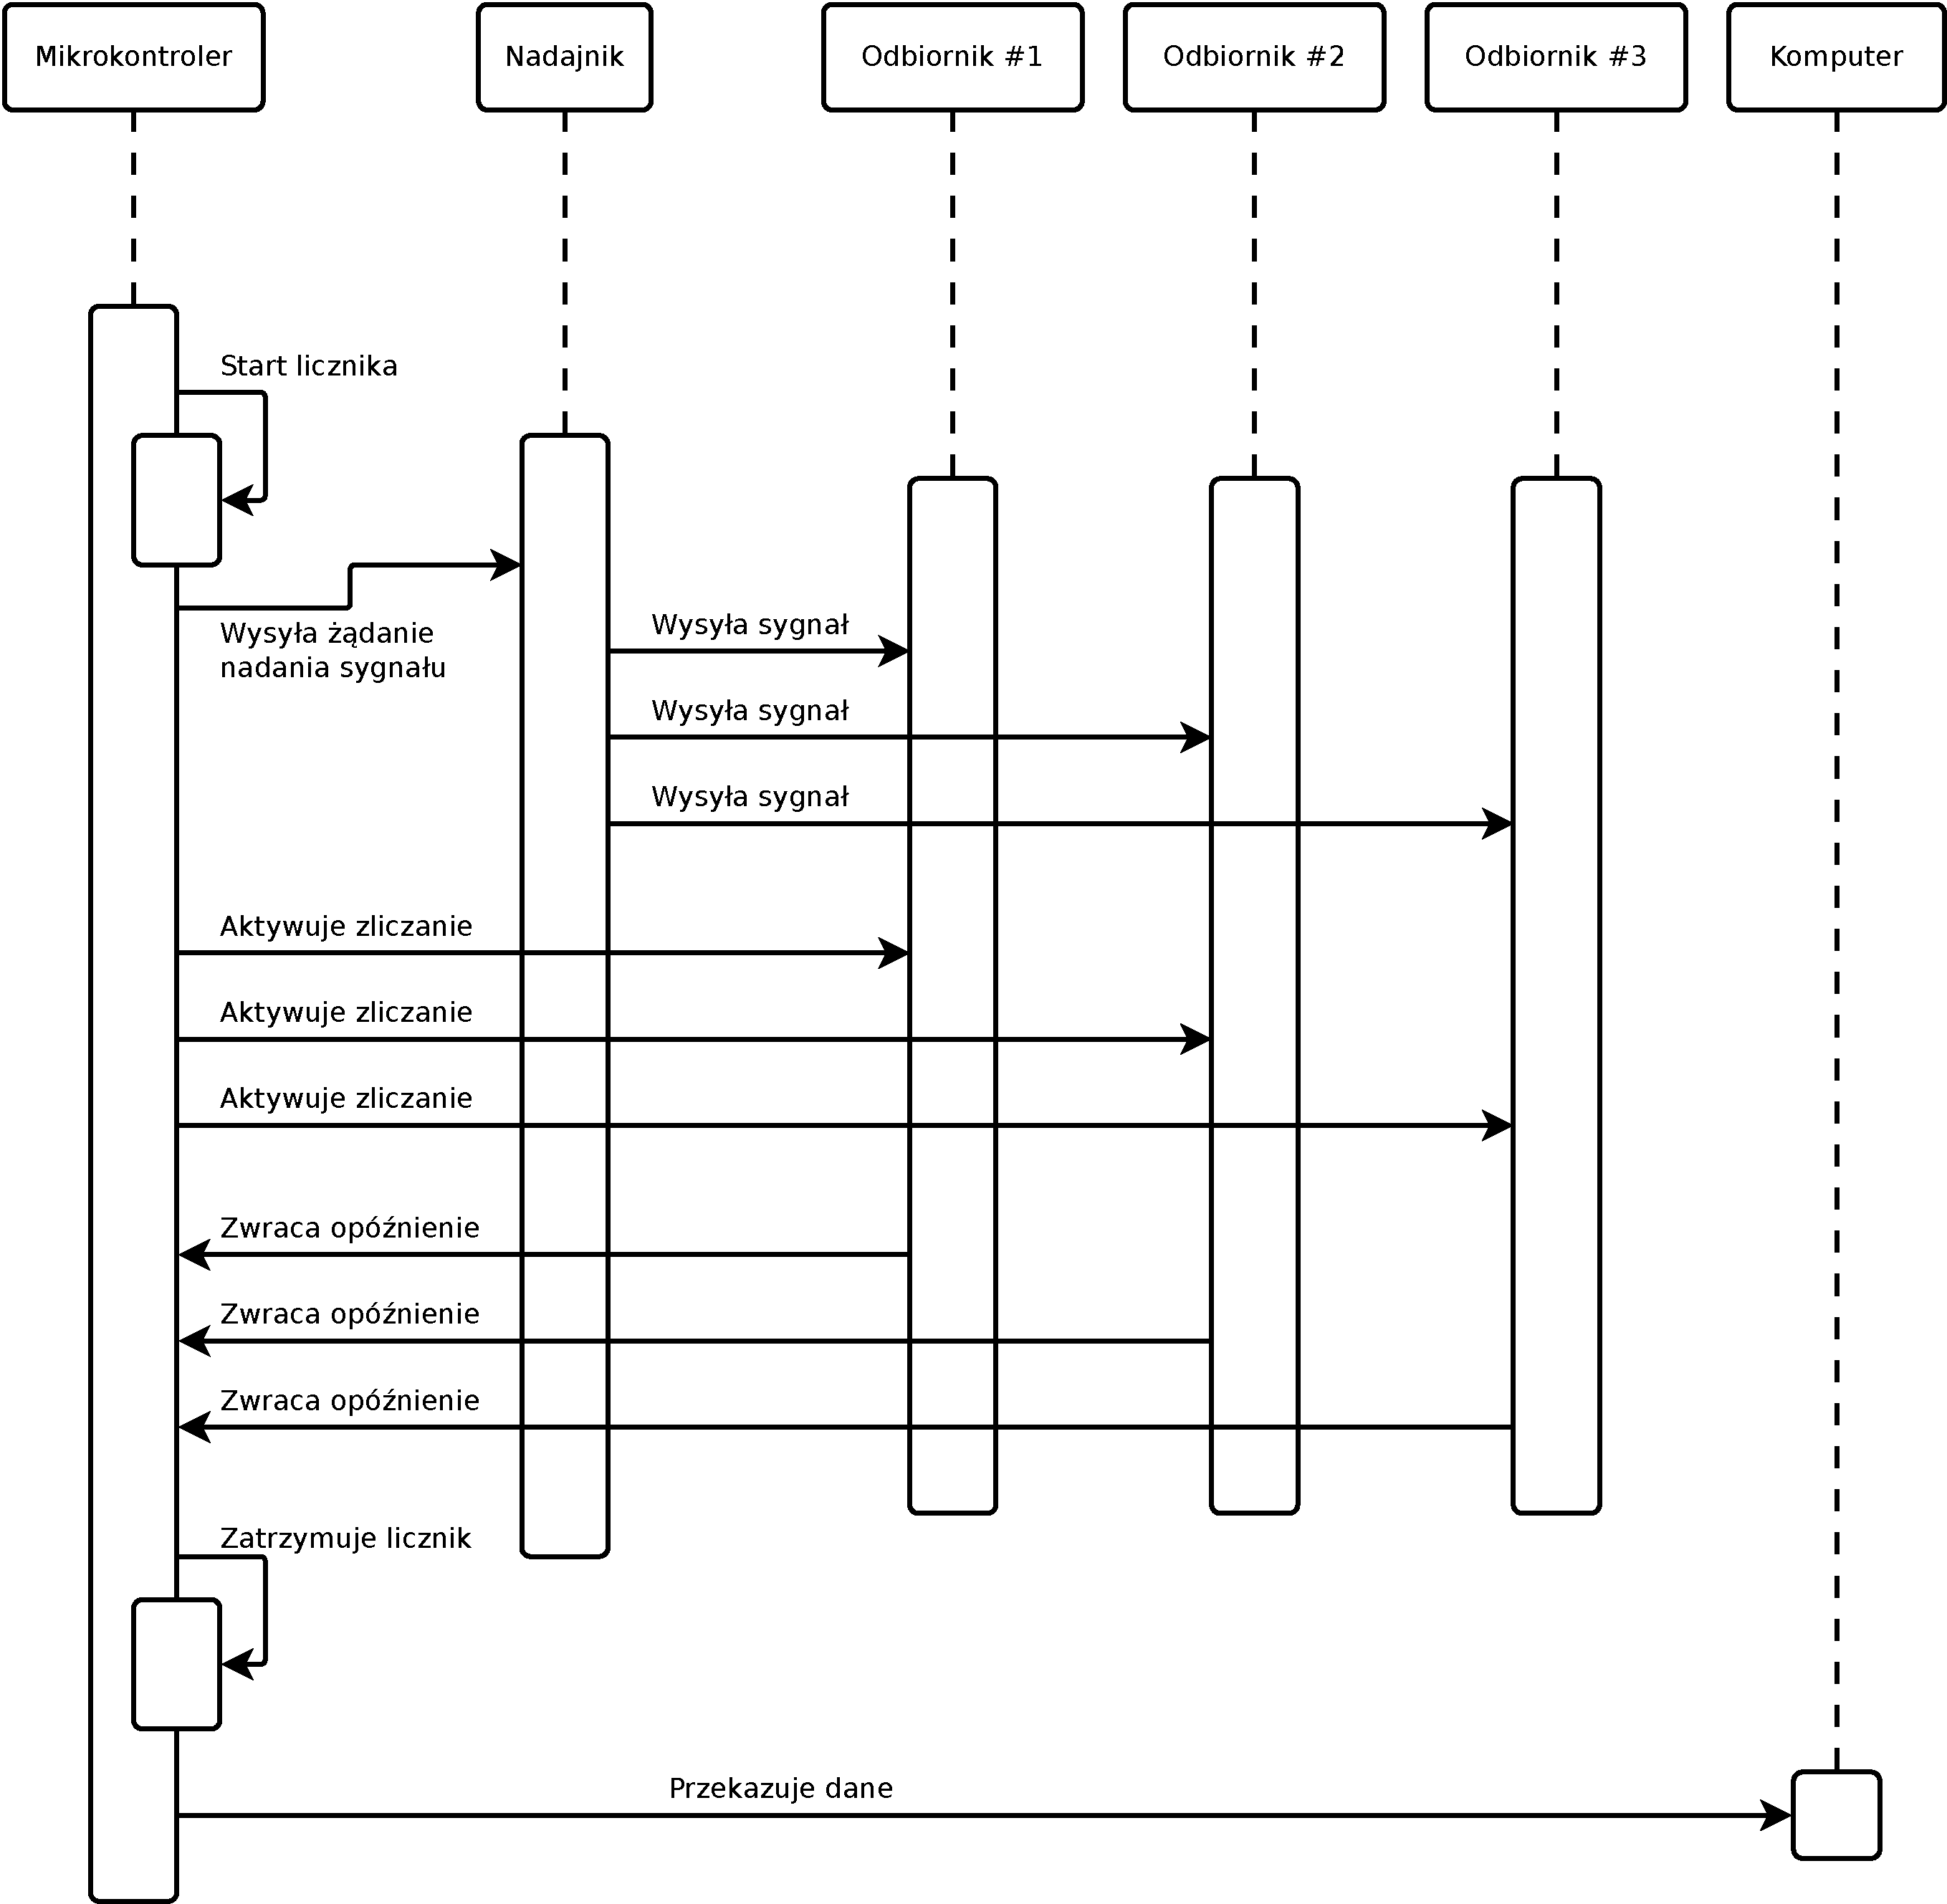
\includegraphics[width=45em]{gfx/diagramy/diagram_sekwencji_sprzetu.pdf}
 \caption{Diagram sekwencji oprogramowania mikrokontrolera}
 \label{fig:firmware_sequence_diagram}
\end{figure}

\paragraph{Prescaler}
W mikrokontroler wbudowany jest \index{prescaler}\textsl{prescaler}, czyli dzielnik częstotliwości, o programowanym stopniu podziału. Jego działanie polega na zliczaniu taktów zegara; gdy wewnętrzny licznik prescalera osiągnie zaprogramowaną wcześniej wartość, wyzwalane jest przerwanie timera oraz następuje przepełnienie licznika, w związku z czym zliczana wartość ,,przekręca się'' i liczenie rozpoczyna się ponownie od zera.

Punkt \ref{enum:prescaler} algorytmu jest bardzo istotny, gdyż nie ma możliwości\graffito{Nawet gdyby możliwość odczytania tej wartości istniała, działanie to wprowadzałoby niepożądane opóźnienia} sprawdzenia aktualnego stanu licznika prescalera, natomiast rozpoczęcie odliczania może nastąpić w dowolnym momencie czasu, przez co może być niekoniecznie zsynchronizowane z wyzwoleniem przerwania przez prescaler, efektem czego byłyby pomiary, które charakteryzowałyby się pewną zmienną niedokładnością.

\paragraph{Przerwania}
W działaniu programu dużą rolę odgrywają procedury obsługi przerwań (ang. \textsl{ISR \ppauza Interrupt Service Routine}). Są to krótkie fragmenty kodu, które wywoływane są przez mikrokontroler w przypadku zajścia pewnego zdarzenia. Ich użycie pozwala na pewien stopień ,,wielowątkowości'', gdyż (w zależności od ustawienia flag) mogą one przerwać wykonywanie głównego toku programu do momentu, aż przerwania nie zostaną ,,obsłużone'', tzn. instrukcje zawarte w procedurze ISR nie zostaną wykonane.

Implementacja procedur obsługi przerwań jest rozszerzeniem języka C, która jest charakterystyczna dla wykorzystanej rodziny układów i wykorzystanego kompilatora, co powoduje, że wykorzystanie innego kompilatora lub innej rodziny układów wymaga przepisania procedur ISR zgodnie z nowymi wymaganiami.

Jednym z wykorzystanych przerwań jest przerwanie wywoływane przez moduł \texttt{Timer/Counter0}: \texttt{Timer/Counter0 Overflow} (\texttt{TOV0}). Jest ono wyzwalane, gdy licznik \texttt{TCNT0} przekroczy maksymalną możliwą dla niego wartość i rozpocznie się ponowne odliczanie od zera. Zadaniem zawartego w tej procedurze kodu jest tylko i wyłącznie inkrementacja zmiennej \texttt{ovfCounter}, dzięki czemu znana jest ilość przepełnień licznika. W przypadku pominięcia tej danej, pomiary ograniczony byłyby do zaledwie 256 możliwości odległości markera od odbiornika.

Drugie wykorzystane przerwanie jest również przerwaniem licznika i wyzwalane jest przez moduł \texttt{Timer/Counter1}. Jedynym zadaniem tego przerwania jest obsługa jednej z diod, której zadaniem jest wizualne potwierdzenie sprawności i działania układu.

Przykład procedury obsługi przerwania na podstawie opisanej właśnie funkcjonalności prezentuje listing~\ref{lst:interrupt_handler}.

\begin{listing}
  \lstinputlisting[language=C]{testy/atmega_interrupt.c}
  \caption{Procedura obsługi przerwania \texttt{Timer/Counter0 Overflow}}
  \label{lst:interrupt_handler}
\end{listing}

Oznaczenie zmiennej jako \texttt{volatile} oznajmia kompilatorowi, że wszelkie odczyty i zapisy muszą operować na wartości zmiennej z pamięci. W przypadku braku takiego zapisu kompilator podczas kompilowania kodu źródłowego z włączoną flagą optymalizacji może przyjąć, że procedura zmieniająca wartość zmiennej nie jest nigdzie wywoływana, przez co bezpiecznym jest cache-owanie wartości zmiennej, a w efekcie zignoruje skutki wywołania przerwania.

Makro \texttt{ISR(vector [, attributes])} z biblioteki \textsmaller{avr-libc} definiuje następujące po nim ciało funkcji jako procedurę obsługi przerwania. Argument \texttt{vector} jest wymagany i oznacza pozycję w wektorze przerwań mikrokontrolera, do której przypisany ma zostać kod. Argument \texttt{attributes} jest opcjonalny i modyfikuje działanie procedury ISR \ppauza pozwala np. na zagnieżdżanie przerwań, czyli przerwanie przetwarzania procedury ISR przez inne przerwanie.

Wygenerowany wektor przerwań, prezentujący obecność tylko dwóch, wymienionych powyżej, procedur obsługi przerwania prezentuje listing~\ref{lst:interrupt_vector}.

\begin{listing}
  \lstinputlisting{testy/interrupt_vector.txt}
  \caption[Wektor obsługi przerwań]{Wygenerowany wektor obsługi przerwań}
  \label{lst:interrupt_vector}
\end{listing}

Pierwsza pozycja na liście jest punktem wejścia programu, od którego rozpoczyna się wykonywanie kodu. Pozycje z adresów \texttt{0x10} i \texttt{0x12} to przekierowania do odpowiednio procedur ISR dla przerwań \texttt{Timer/Counter0 Overflow} i \texttt{Timer/Counter1 Overflow}.

\section{Oprogramowanie dla komputera}
W celu stworzenia oprogramowania dla komputera wykorzystałem kilka środowisk i bibliotek.

\paragraph{Qt}
Wieloplatformowe środowisko \textsmaller{Qt} składa się z kilku komponentów. W jego skład wchodzą między innymi:
\begin{description}
 \item[biblioteka Qt] skompilowane źródła, z których korzysta aplikacja podczas uruchamiania
\end{description}


\subsection{Trilaterator}
Pierwsza ze stworzonych aplikacji przeznaczona jest do przeprowadzania trilateracji, o której mowa w sekcji \ref{par:trilateration}. Wykonuje ona automatycznie obliczenia dane wzorami \ref{eq:trilateration_final_x}, \ref{eq:trilateration_final_y} i \ref{eq:trilateration_final_z}. Interfejs aplikacji umożliwia wprowadzanie wszelkich danych dotyczących rozmieszczenia odbiorników jak i markera. Wyniki dokonanych obliczeń prezentowane są w dolnej części programu.

Aplikację wraz z przykładowymi danymi prezentuje rysunek \ref{fig:trilaterator}.

Przykładowe dane oraz poprawność zastosowanej metody pokazuje rysunek \ref{fig:trilateration_sample}.

Jak widać, oddalenie odbiorników od siebie na odległość zaledwie kilku centymetrów pozwala badać położenie markera w przestrzeni.

\paragraph{Struktura programu}
Przedstawiony program jest celowo bardzo prosty i sprowadza się tylko do obsługi zdarzenia kliknięcia przycisku, tak aby łatwo można było prześledzić działanie metody. Całą istotę działania programu prezentuje listing~\ref{lst:trilateration}.

\begin{listing}
  \lstinputlisting{testy/trilateration.cpp}
  \caption{Kod dokonujący trilateracji}
  \label{lst:trilateration}
\end{listing}

\paragraph{Dokładność obliczeń}
Należy wziąć pod uwagę fakt, że odległość pomiędzy odbiornikami ma wpływ na wynik obliczeń. Wynika to z operowania przez komputer na danych o skończonej i zmiennej dokładności.

Jeśli marker znajdzie się dostatecznie daleko od odbiorników, może nastąpić spadek precyzji, gdyż dane są reprezentowane w pamięci komputera przez typy zmiennoprzecinkowe i przy małym rozsunięciu odbiorników po wykonaniu działań arytmetycznych, a w szczególności operacji potęgowania i pierwiastkowania, jakie są konieczne do odtworzenia pozycji, utrata precyzji będzie miała znaczący wpływ na wynik obliczeń.

Aby uniknąć tego problemu, odbiorniki \textsl{Nietoperza} rozstawione są na planie trójkąta równobocznego o boku 33cm. Pozwala to na wystarczająco dokładne śledzenie precyzji już za pomocą typu zmiennoprzecinkowego pojedynczej precyzji \verb|float|. Na potrzeby tej demonstracji zdecydowałem się jednak wykorzystać typ dostarczający podwójnej precyzji \verb|double|.

\paragraph{Wieloplatformowość}
Aplikacja ta prezentuje także zalety wykorzystanego środowiska, które może być kompilowane pod wszystkimi trzema znaczącymi systemami: \textsl{Linux}, \textsl{Windows} i \textsl{Mac OS X}. Do poprawnego skompilowania nie jest wymagana żadna zmiana kodu.

\begin{figure}
 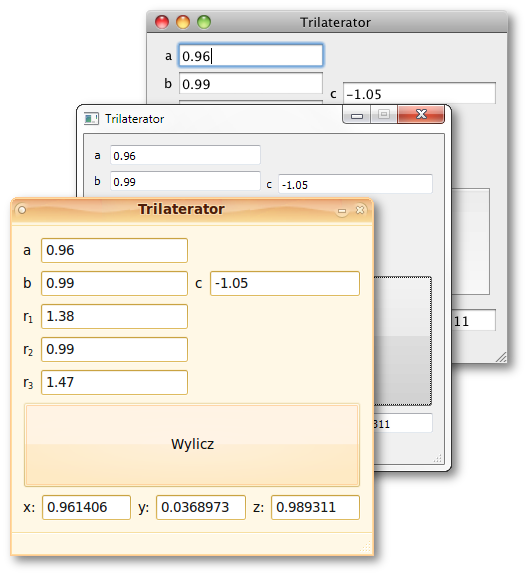
\includegraphics[width=\textwidth]{gfx/trilaterator_triple.png}
 \caption{Trilaterator. Aplikacja dokonująca trilateracji}
 \label{fig:trilaterator}
\end{figure}

\begin{figure}
  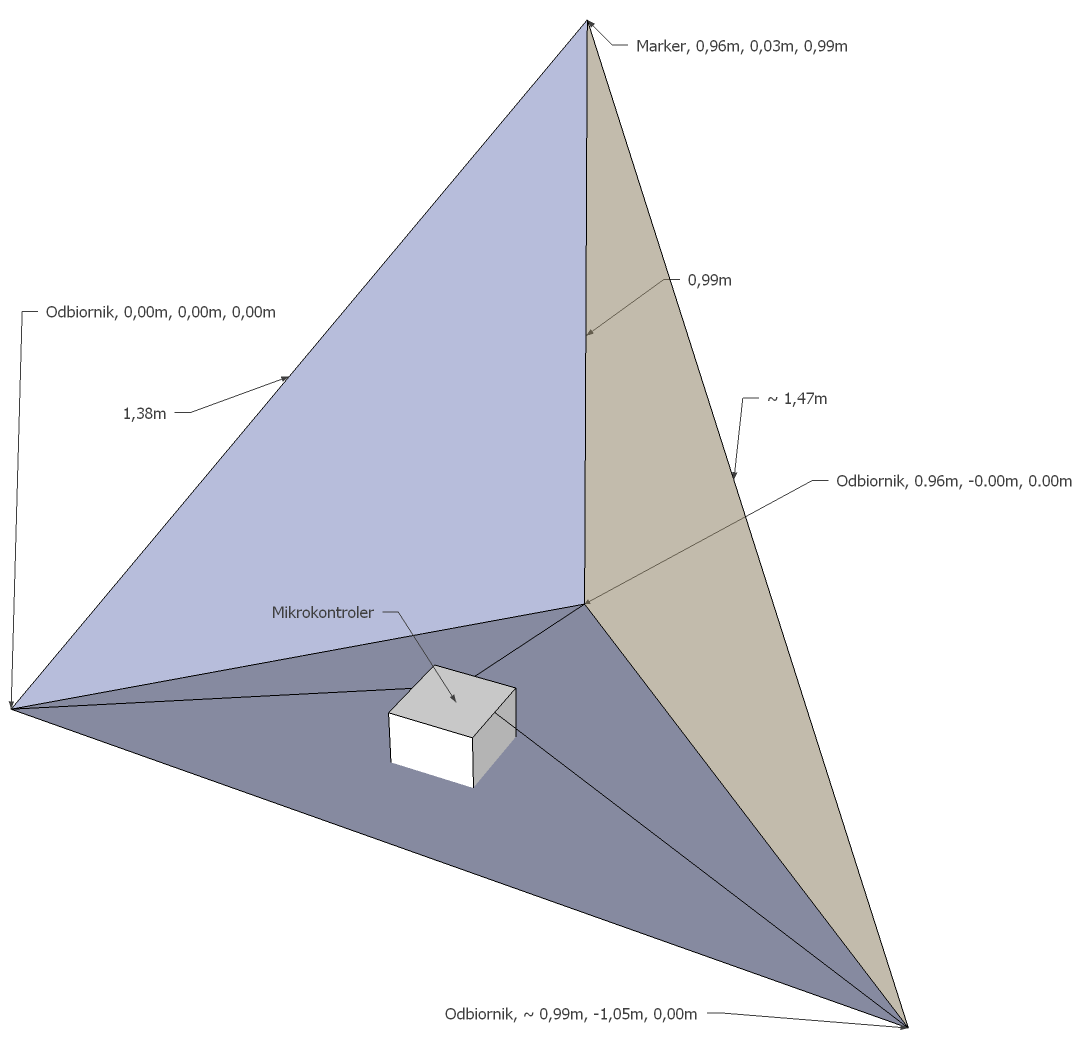
\includegraphics[width=\textwidth]{gfx/wizualizacja_3d.png}
  \caption{Wizualizacja przykładowych danych}
  \label{fig:trilateration_sample}
\end{figure}

\begin{figure}
 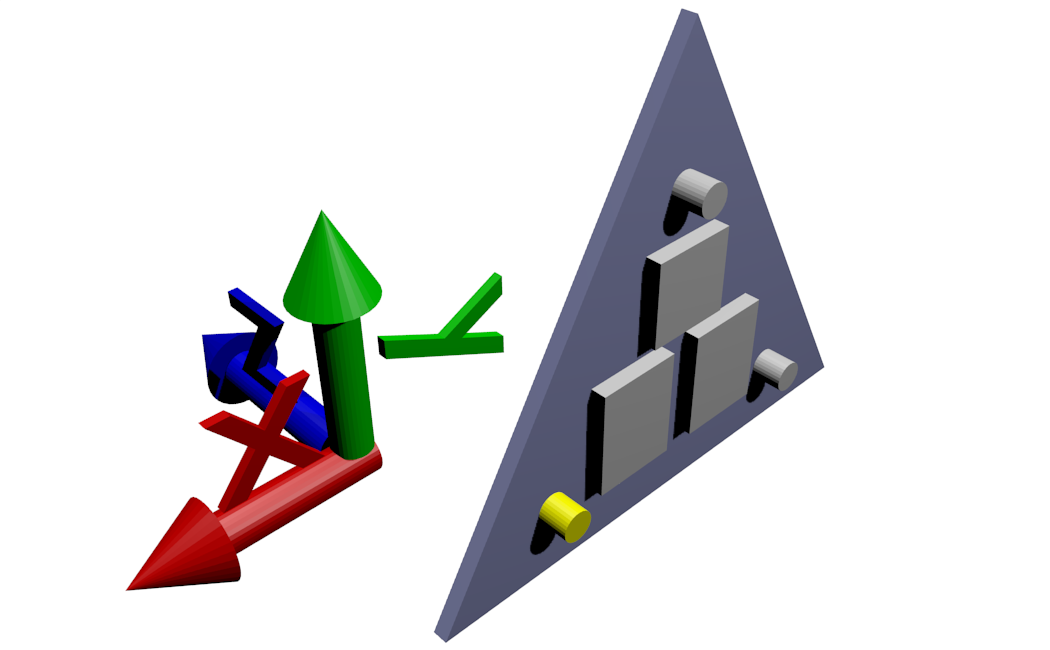
\includegraphics[width=\textwidth]{gfx/uklad_render.png}
 \caption[Model systemu i przyjęty układ współrzędnych]{Model systemu wraz z przyjętym układem współrzędnych. Układ ma swój początek w odbiorniku oznaczonym kolorem żółtym}
 \label{fig:coordinate_system}
\end{figure}

\subsection{Charter}
Kolejna aplikacja prezentująca możliwości systemu służy do rysowania wykresów w czasie rzeczywistym na podstawie danych pobranych z mikrokontrolera. Dla porównania dostępne są dwa rodzaje wykresów jednocześnie:
\begin{itemize}
 \item odległość od odbiornika \ppauza pokazuje odległość wybranego markera od każdego z odbiorników,
 \item położenie \ppauza dokonuje w locie trilateracji dla bieżącej próbki i rysuje wykres położenia wybranego markera w trzech wymiarach, zgodnie z układem odniesienia przedstawionym na rysunku \ref{fig:coordinate_system}.
\end{itemize}

Odległość od odbiorników podawana jest jako wartość licznika odczytana z mikrokontrolera. Aby dokonać konwersji na centymetry, należy (w oparciu o równanie \ref{eq:microcontroller_limit}) przeliczyć:
\begin{equation}
 d = \frac{x \cdot 0,34\textrm{mm}}{10}
\end{equation}
gdzie:
\begin{description}
 \item[$d$] \ppauza~wyznaczona odległość w centymetrach,
 \item[$x$] \ppauza~odległość odczytana z wykresu.
\end{description}

Użytkownik w trakcie działania programu ma możliwość wyboru, którego markera dane powinny być rysowane.

Program dokonuje transformacji układu współrzędnych, aby w efekcie uzyskać układ pokazany na rysunku \ref{fig:coordinate_system}.

Jest to taki sam prawoskrętny układ, jak wykorzystywany w bibliotece \textsc{OpenGL}, co znacząco ułatwia pracę, ponieważ nie jest wymagana żadna dodatkowa konwersja układu współrzędnych aby narysować pozycję markera.

\paragraph{Struktura programu}

\paragraph{Rozszerzanie obsługi o dodatkowe markery}
\makeatletter @ \makeatother
Chociaż dostępne aktualna wersja sprzętu zaproejtkowana jest do obsługi tylko i wyłącznie dwóch markerów, to prezentowany program przygotowany został w sposób pozwalający na obsługę dowolnej ilości markerów.

Zadbałem o to, aby dodawanie markerów było możliwie proste dla programisty. Wykorzystałem w tym celu mało znaną możliwość, jaką oferuje środowisko \textsc{Qt}, tj. jawne wykorzystanie meta-obiektów\graffito{dodać info o moc}.

Deklarując próbkę jako klasę \verb|Sample|, która dziedziczy z podstawowej klasy środowiska \textsc{Qt}, \verb|QObject|, możliwe jest pozyskanie w czasie działania programu (ang. \textsl{runtime}) dostępu do pewnych danych, które w innym przypadku byłyby niedostępne lub dostęp do nich wymagałby od programisty dużej gimnastyki, a nawet wykorzystania bibliotek trzecich takich jak np. \textsc{Boost}.

Podejście takie wymusiło na mnie jednak dostarczenie publicznych implementacji konstruktora domyślnego, konstruktora kopiującego oraz operatora przypisania:
\begin{verbatimtab}
public:
	Sample(QObject *parent = 0);
	Sample(const Sample &other);
	Sample &operator =(const Sample &other);
\end{verbatimtab}
gdyż w klasie \verb|QObject| są to metody prywatne, co uniemożliwia wykorzystywane w kodzie programu kopiowanie i tworzenie automatycznych zmiennych tego typu.

Jedną z możliwości środowiska \textsc{Qt} jest zarejestrowanie typu wyliczeniowego \verb|enum| w systemie meta-obiektów poprzez wywołanie makra \verb|Q_ENUMS|:
\begin{verbatimtab}
class Sample : public QObject
{
	Q_OBJECT;
	Q_ENUMS(Marker);
public:
	enum Marker {Blue = 1, Yellow = 2};
	(...)
\end{verbatimtab}

Działanie to pozwala na dostęp do tak zarejestrowanego typu \verb|enum| w działającym programie za pomocą meta-właściwości. Możliwe jest nie tylko poznanie zarejestrowanych w klasie typów, ale także iteracja przez zarówno klucze, jak i właściwości.

Wykorzystanie tej cechy powoduje, że do dodania dodatkowego markera jedyne wymagania, jakich spełnienie musi zapewnić programista to:
\begin{aenumerate}
  \item dodanie identyfikatora markera do typu \verb|Sample::Marker|,
  \item poprawienie kodu wątku obsługującego odczytywanie danych, aby obsłużył zmodyfikowany protokół.\label{item:modify_protocol}
\end{aenumerate}

Jeśli protokół nie zostanie zmieniony, to punkt \ref{item:modify_protocol} nie jest wymagany.

Jak widać dodanie nowego markera jest zadaniem trywialnym.

Chociaż kosztem łatwości rozszerzalności oprogramowania wymaganych jest kilka wywołań funkcji więcej, to nie ma to znaczącego wpływu na wydajność programu.

\section{Protokół}
\label{sec:protocol}
\index{protokół}
Mikrokontroler komunikuje się z komputerem za pomocą standardu \index{RS232}\textsmaller{RS232}, do obsługi którego wykorzystuje moduł \index{USART}\textsmaller{USART}. Aby uzgodnić dane pomiędzy komputerem a mikrokontrolerem, zaprojektowałem protokół, zgodnie z którym następuje przekazanie danych.

Protokół taki powinien zawierać możliwie mało nadmiarowych danych, umożliwiać synchronizację bez względu na moment włączenia nadajnika (mikrokontrolera) względem odbiornika (komputera) oraz zawierać wszystkie potrzebne informacje do odtworzenia położenia wszystkich obsługiwanych markerów.

Mianem \index{raport}\emph{raportu} będziemy nazywać jeden pełen zestaw danych, jakie przesyła do komputera mikrokontroler.

Raport w zaprojektowanym protokole prezentuje rysunek \ref{fig:protocol}.

\begin{figure}
 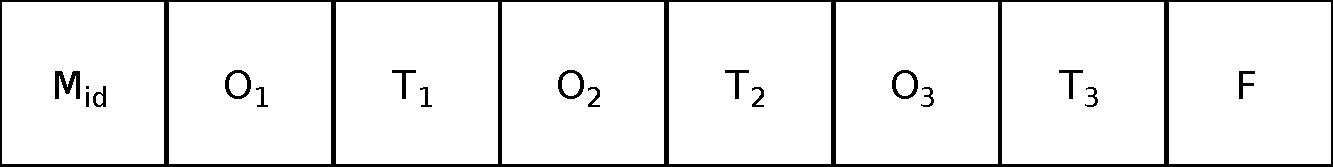
\includegraphics[width=\textwidth]{gfx/diagramy/protokol.pdf}
 \caption[Schemat raportu]{Raport w protokole komunikacji mikrokontrolera z komputerem}
 \label{fig:protocol}
\end{figure}

Każda ramka składa się z ośmiu bajtów, do których należą:
\begin{itemize}
 \item \texttt{M$_\textrm{\texttt{id}}$} \ppauza $id$ markera,
 \item \texttt{O$_n$} \ppauza wartość zmiennej \texttt{ovfCounter} w chwili wygaszenia pinu odbiornika $n$,
 \item \texttt{T$_n$} \ppauza wartość rejestru \texttt{TCNT0} w chwili wygaszenia pinu odbiornika $n$,
 \item \texttt{F} \ppauza zawsze \texttt{0xFF}.
\end{itemize}

Pole \texttt{F} wraz z polem \texttt{M$_\textrm{\texttt{id}}$} służy do synchronizacji danych odbieranych przez komputer. Metodę \index{synchronizacja}synchronizacji prezentuje algorytm \ref{alg:sync}.

\begin{algorithm}
\caption{Metoda synchronizacji danych}
\label{alg:sync}
\begin{algorithmic}[1]
  \REQUIRE \texttt{dane} \ppauza tablica dynamiczna, do której końca dopisywane są przychodzące dane
  \WHILE{\texttt{dane.count() $\geq$ 8}}
    \WHILE{\texttt{dane.count() $\geq$ 8 \&\& (dane[0] != M$_\textrm{\texttt{id}}$ \textbar{}\textbar{} dane[7] != 0x77})}
      \STATE usuń(\texttt{dane[0]})
    \ENDWHILE
  \ENDWHILE
\end{algorithmic}
\end{algorithm}

Należy zauważyć, że poza samymi danym protokołu, pomiędzy kompterem, a mikrokontrolerem przekazywane są również dane kontrolne standardu \index{RS232}RS232:
\begin{itemize}
  \item bity startu,
  \item bity stopu.
\end{itemize}

Zrezygnowałem natomiast z funkcji:
\begin{itemize}
 \item bity parzystości \ppauza te dane kontrolne bardzo słabo spełniają swoją rolę, gdyż są bardzo podatne na zakłócenia, które powodują przestawienie parzystej ilości bitów,
 \item kontrola przepływu \ppauza funkcjonalność nie jest dostępna w mikrokontrolerze.
 \item więcej niż 8 bitów w jednej ramce \ppauza chociaż mikrokontroler oferuje przesłanie do 9 bitów danych w jednej ramce, to wykorzystanie tej funkcjonalności znacznie ograniczyłoby funkcjonalność platformy ze względu na fakt, iż układy stosowane w komputerach rzadko kiedy oferują obsługę takich ramek\graffito{Obsługa 9-bitowych ramek wymaga też specjalnego oprogramowania}, ponadto spowodowałoby dodatkowy narzut pracy na mikrokontrolerze związany z podziałem danych na 9-bitowe części, nie oferując przy tym żadnego wzrostu wydajności \ppauza przesłanie 64 bitów wymagałoby i tak 8 ramek.
\end{itemize}

Pełna ramka standardu RS232 składa się zatem z 10 bitów:
\begin{enumerate}
 \item bit startu,
 \item 8 bitów danych,
 \item bit stopu.
\end{enumerate}